% Тут используется класс, установленный на сервере Papeeria. На случай, если
% текст понадобится редактировать где-то в другом месте, рядом лежит файл matmex-diploma-custom.cls
% который в момент своего создания был идентичен классу, установленному на сервере.
% Для того, чтобы им воспользоваться, замените matmex-diploma на matmex-diploma-custom
% Если вы работаете исключительно в Papeeria то мы настоятельно рекомендуем пользоваться
% классом matmex-diploma, поскольку он будет автоматически обновляться по мере внесения корректив
%

% По умолчанию используется шрифт 14 размера. Если нужен 12-й шрифт, уберите опцию [14pt]
\documentclass[14pt]{matmex-diploma}
%\documentclass[14pt]{matmex-diploma-custom}
\usepackage{listing}
\usepackage{float}

\begin{document}
% Год, город, название университета и факультета предопределены,
% но можно и поменять.
% Если англоязычная титульная страница не нужна, то ее можно просто удалить.
\filltitle{ru}{
    chair              = {Кафедра Системного программирования},
    title              = {Разработка архитектуры для унификации синтаксических анализаторов в проекте YaccConstructor},
    % Здесь указывается тип работы. Возможные значения:
    %   coursework - Курсовая работа
    %   diploma - Диплом специалиста
    %   master - Диплом магистра
    %   bachelor - Диплом бакалавра
    type               = {coursework},
    position           = {студента},
    group              = 344,
    author             = {Соловьев Александр Александрович},
    supervisorPosition = {ст. преп., к.\,ф.-м.\,н.},
    supervisor         = {Григорьев С.\,В.}
}
\maketitle
\tableofcontents

\section*{Введение}
Основной задачей синтаксического анализа является задача проверки выводимости некоторой последовательности токенов в заданной грамматике и построением соответствующего дерева вывода. Данная задача может быть рассмотрена шире, так как в качестве объекта синтаксического анализа могут рассматриваться структуры данных, отличные от последовательностей. Так, в работах \cite{graphParseVerb} и \cite{graphParseRag} синтаксическому анализу подвергается граф.

В 2010 году был представлен алгоритм обобщенного синтаксического анализа Generalized LL (GLL), в основе которого лежит алгоритм нисходящего синтаксического анализа~\cite{GLLParsing}. Данный алгоритм и различные его модификации были реализованы в проекте YaccConstructor~\cite{YaccConstructor} в качестве отдельных не связанных между собой модулей (рис. \ref{fig:Old})). Различаются они в структурах, представляющих входные данные, в представлении вспомогательных структур и в возможности построения деревьев вывода. В то время, как основная структура различных версий алгоритма неизменна, внутрення их реализация различна в зависимости от используемых структур и необходимости построения деревьев вывода. Несмотря на то, что алгоритмы в большей части одинаковы, их поддержка и сопровождение затруднены в связи с независимостью реализаций. Данную проблему возможно решить их обобщением. Теоретически оно возможно, однако на практике может привести к возникновению различных трудностей, получившееся решение может оказаться настолько более сложным, что его сопровождение окажется еще более проблематичным, чем сопровождение всего набора независимо реализованных алгоритмов. Наиболее вероятным недостатком может оказаться значительное падение производительности. Так представление последовательности токенов в виде графа ведет к появлению циклов перебора всех исходящих из вершины ребер, что ведет к росту числа операций.

\section{Постановка задачи}
Целью данной работы является разработка архитектуры для унификации существующих синтаксических анализаторов в проекте \newline YaccConstructor. Для достижения данной цели были поставлены следующие задачи:
\begin{itemize}
    \item спроектировать архитектуру, позволяющую объединить различные модификации алгоритма;
    \item реализовать предложенную архитектуру;
    \item разработать тестовое покрытие;
    \item провести эксперименты для оценки производительности.
\end{itemize}

\section{Обзор}
\subsection{YaccConstructor}
YaccConstructor --- проект, разрабатываемый в лаборатории языковых инструментов JetBrains, расположенной на кафедре системного программирования. В нем занимаются исследованиями и разработками в области лексического и синтаксического анализа. Большинство компонентов проекта реализованы на языке F\#, исходный код проекта находится в открытом доступе \cite{YaccConstructor}. Проект имеет модульную архитектуру (рис.\ref{fig:YCArch}), что позволяет собирать требуемый инструмент из существующих модулей: можно выбрать фронтенд, задать требуемые преобразования грамматики и указать генератор. Фронтенды позволяют построить по спецификации грамматики ее внутреннее представление, к которому могут быть применены необходимые преобразования, генераторы предоставляют инструменты, позволяющие по внутреннему представлению грамматики получить нужный пользователю результат, например, таким результатом может быть синтаксический анализатор.

\begin{figure}[h]
	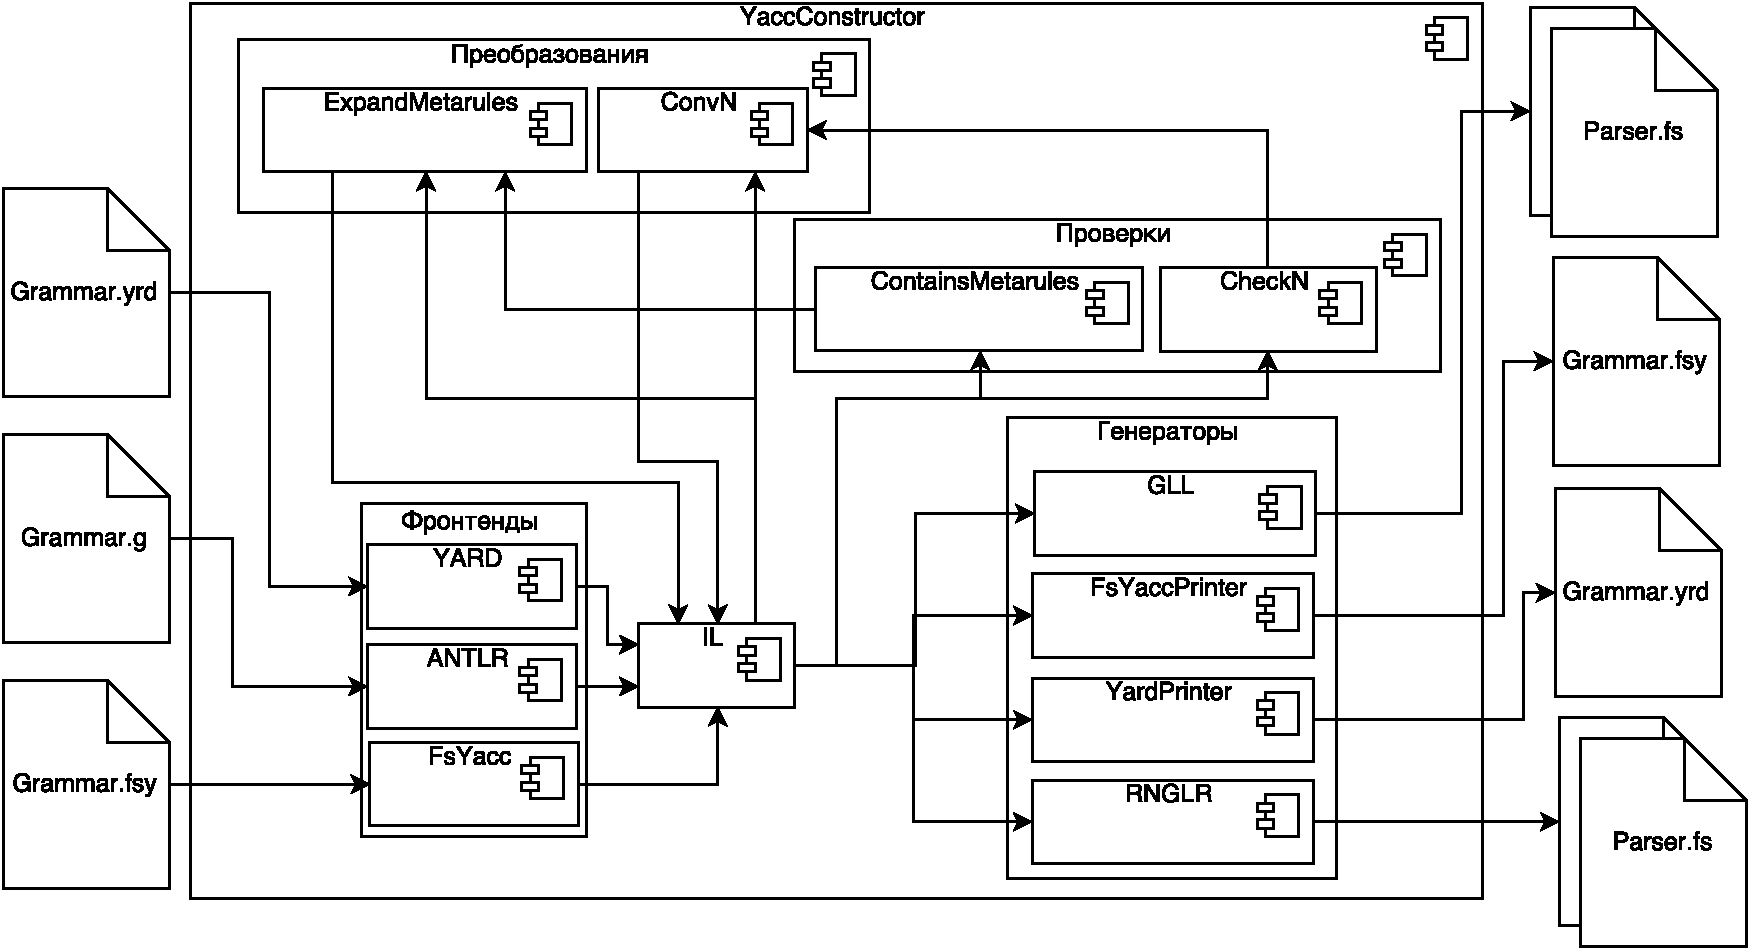
\includegraphics[width=\textwidth]{images/YCArch}
	\caption{Архитектура YaccConstructor, заимствована из \cite{gsvPhd}}
	\label{fig:YCArch}
\end{figure}

\subsection{Синтаксические анализаторы на основе GLL}
Как говорилось выше, в проекте было реализовано несколько модификаций GLL, различавшихся в том, подавались ли на вход алгоритму грамматика или же рекурсивный автомат \cite{RADesc}, в объекте синтаксического анализа, а также в возможности построения дерева.

\subsubsection{Generalized LL}
GLL имеет некоторые преимущества перед прочими алгоритмами синтаксического анализа:
\begin{itemize}
    \item разбор любых контекстно-свободных грамматик, в том числе и неоднозначных;
    \item время исполнения в худшем случае кубически зависит от размера входных данных;
    \item алгоритм обладает свойством "рекурсивного спуска": анализатор может быть легко построен напрямую по грамматике.
\end{itemize}
В 2013 году была представлена статья \cite{GLLTreeGen}, в которой описывалось конструирование структуры SPPF (Shared Packed Parse Forest) в ходе работы GLL. SPPF представляет все возможные деревья вывода строки в заданной грамматике.

\subsubsection{Синтаксический анализ графов}
При решении различных практических задач может возникнуть необходимость проверки выводимости элементов некоторого регулярного множества в заданной грамматике. Подобное множество может быть и бесконечным, в таком случае проверка всех его элементов на выводимость не представляется возможной. Однако, поскольку регулярные множества описываются при помощи конечных автоматов, задачу можно свести к проверке выводимости элементов, заданных конечным автоматом в заданной грамматике. Примером подобной задачи может стать проверка корректности динамически формируемых SQL-запросов.

\subsubsection{Использование рекурсивного автомата}
\label{subsec:ra}
Процесс конструирования синтаксических анализаторов может быть автоматизирован с помощью генераторов при наличии требуемой спецификации. Предствленая она может быть в расширенной форме Бэкуса-Наура, справиться с которой способны немногие решения, однако они не умеют работать с неоднозначными грамматиками. В работе \cite{paperFSA} представлена модификация GLL, позволяющая работать с грамматиками в форме, близкой к РФБН. Также показано, что данное решение имеет лучшую проивзодительность, чем при трансформации грамматики.

\newpage
\subsection{Изначальная архитектура}
Как уже говорилось, основной проблемой данной архитектуры (рис. \ref{fig:Old}) являлась проблематичность ее сопровждения, что следовало из целого ряда ее недостатков. Одним из самых серьезных недостатков является то, что используемые алгоритмами структуры данных, основными из которых являются GSS и SPPF не были выделены в отдельные сущности и реализовывались для каждого алгоритма отдельно с незначительными изменениями. Некоторые структуры данных все же использовались какой-либо группой алгоритмов, но при этом, как правило, имелись структуры данных, испольнявшие аналогичные роли, но в других группах алгоритмов. Последнее приводило к тому, что при изменении таких структур данных изменению также должны были подвергнуться и использовавшие ее алгоритмы. Многое из сказанного выше было справедливо и для функций.
\begin{figure}[H]
    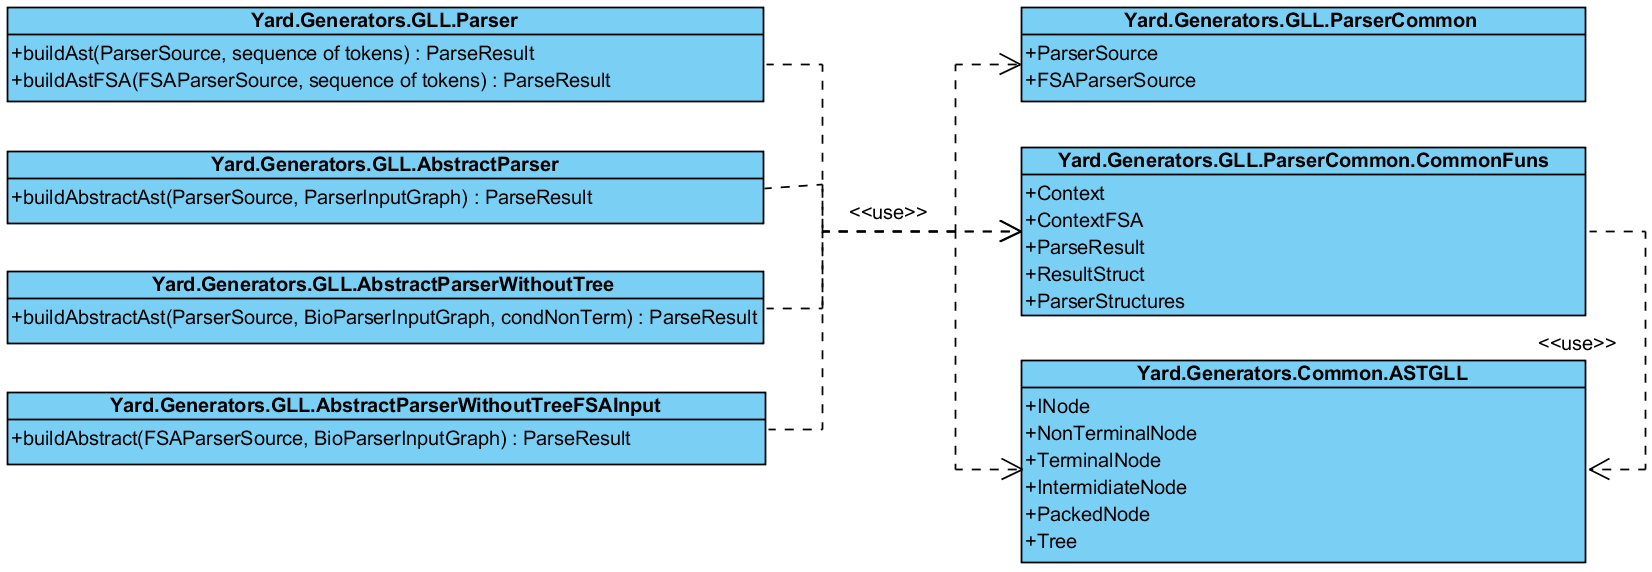
\includegraphics[width=\textwidth]{images/Old}
    \caption{Взаимодействие основных модулей при изначальной архитектуре}
    \label{fig:Old}
\end{figure}

\section{Новая архитектура}
Реализованная архитектура позволяет избежать упоямнутых ранее проблем. Структуры GSS (Graph Structured Stack) и SPPF были выделены в отдельные сущности, что позволило снять с алгоритма ответственность за работу с ними. Для различных входных данных было решено использовать абстракцию, конкретные реализации которой ответственны за различные действия над входными данными, что позволило обобщить алгоритм для различных входных данных. Подобное решение обусловленно тем, что различия в действиях над входными данными зависят исключительно от их внутреннего представления. Из-за описанных в разделе \ref{subsec:ra} достоинств рекурсивного автомата было решено использовать его в качестве единственного представления грамматики. Был добавлен флаг, определяющий, будет ли в процессе работы алгоритма строиться дерево вывода. Таким образом осталась только одна версия алгоритма, обобщенная для различных входных данных и умеющая строить дерево при необходимости.
\begin{figure}[h]
    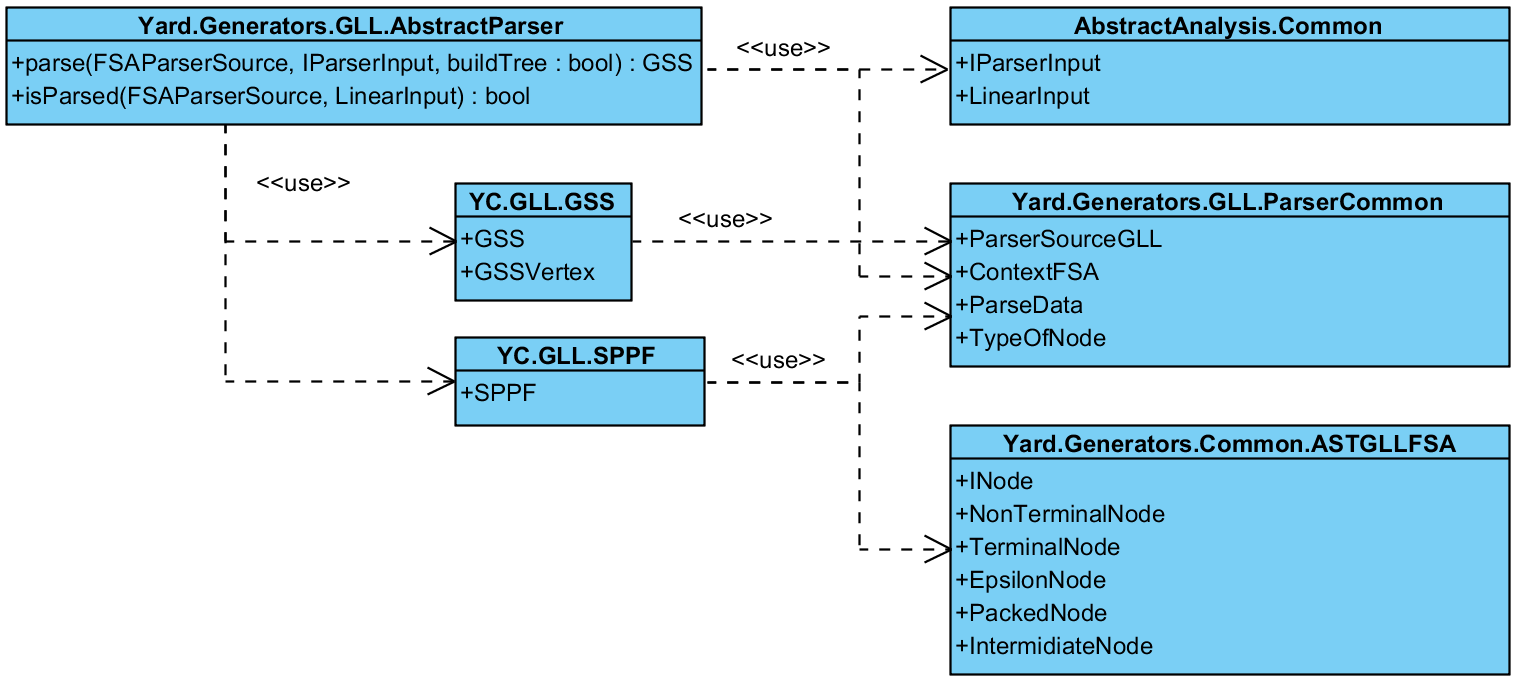
\includegraphics[width=\textwidth]{images/New}
    \caption{Архитектура решения после унификации}
    \label{fig:New}
\end{figure}

\section{Эксперименты}
В рамках данной работы были произведены эксперемнты по сравнению производительности алгоритмов до их обобщения и после.
Замеры производились на компьютере со следующими характеристиками:
\begin{itemize}
    \item Операционная система: Microsoft Windows 10 Home
    \item Тип системы: x64-based PC
    \item Процессор: Intel(R) Core(TM) i7-3630QM CPU @ 2.40GHz, 2.40GHz, 4 Core(s), 8 Logical Processor(s)
    \item Объем оперативной памяти: 8.0 GB
\end{itemize}

\begin{figure}[H]
 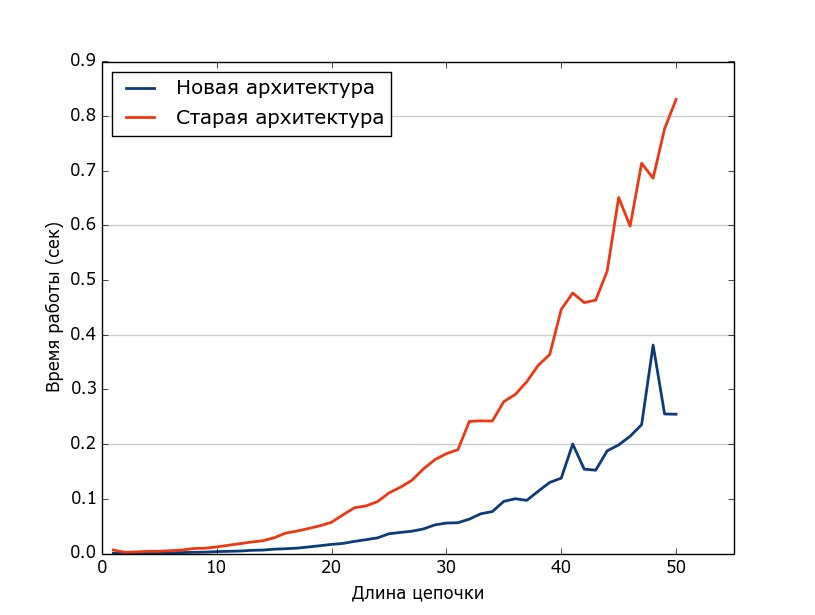
\includegraphics[width=\textwidth]{images/BBB.jpg}
 \caption{Сравнение времени работы старого и нового решения для грамматики $G$}
 \label{exp1}
\end{figure}
Для сравнения были выбраны выбраны две грамматики, первая из которых -- сильно неоднозначная грамматика $G$, реализующая худший случай для анализатора. Результаты измерений представлены на рис.~\ref{exp1}.

\begin{center}
\begin{listing}
$s \rightarrow s \ s \ s \ |  \ s \ s \ | \ B$
\label{grmG}
\caption{Грамматика $G$}
\end{listing}
\end{center}

Следующий эксперимент проводился на грамматике подмножества языка T-SQL \cite{GrammarZoo}. Пример входного графа приведен на рис.~\ref{sqlInput}. Результаты измерений представлены на рис.~\ref{exp2}

\begin{figure}[H]
 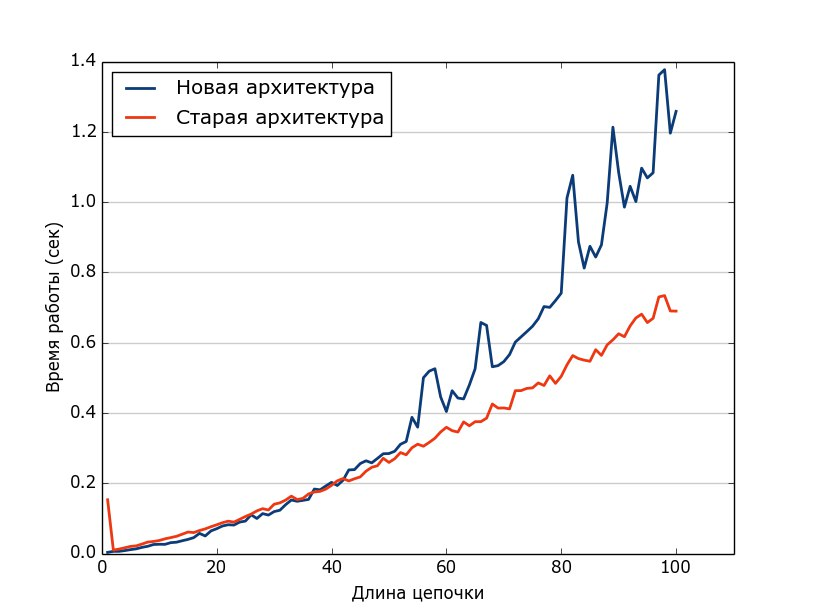
\includegraphics[width=\textwidth]{images/MsSql.jpg}
 \caption{Сравнение времени работы старого и нового решения для грамматики T-SQL}
 \label{exp2}
\end{figure}

\begin{figure}[H]
 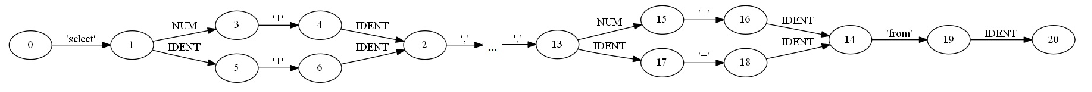
\includegraphics[width=\textwidth]{images/SQLInput.pdf}
 \caption{Структура графа для эксперимента на T-SQL, заимствована из \cite{graphParseRag}}
 \label{sqlInput}
\end{figure}
Результаты экспериментов выше наглядно показывают, что производительность алгоритма осталась на том же уровне, о ее изменении можно судить лишь для конкретных входных данных.

\newpage
\section{Заключение}
Достигнуты следующие результаты:
\begin{itemize}
    \item произведен обзор статей, связанных с предметной областью;
    \item написан обзор предметной области;
    \item спроектирована и реализована архитектура (рис. \ref{fig:New});
    \item разработано тестовое покрытие;
    \item проведены эксперименты для оценки производительности.
\end{itemize}

\setmonofont[Mapping=tex-text]{CMU Typewriter Text}
\bibliographystyle{ugost2008ls}
\bibliography{diploma.bib}
\end{document}
